\documentclass[12pt, twoside]{article}
\documentclass[12pt, twoside]{article}
\usepackage[letterpaper, margin=1in, headsep=0.2in]{geometry}
\setlength{\headheight}{0.6in}
%\usepackage[english]{babel}
\usepackage[utf8]{inputenc}
\usepackage{microtype}
\usepackage{amsmath}
\usepackage{amssymb}
%\usepackage{amsfonts}
\usepackage{siunitx} %units in math. eg 20\milli\meter
\usepackage{yhmath} % for arcs, overparenth command
\usepackage{tikz} %graphics
\usetikzlibrary{quotes, angles}
\usepackage{graphicx} %consider setting \graphicspath{{images/}}
\usepackage{parskip} %no paragraph indent
\usepackage{enumitem}
\usepackage{multicol}
\usepackage{venndiagram}

\usepackage{fancyhdr}
\pagestyle{fancy}
\fancyhf{}
\renewcommand{\headrulewidth}{0pt} % disable the underline of the header
\raggedbottom
\hfuzz=2mm %suppresses overfull box warnings

\usepackage{hyperref}
\usepackage{float}

\title{Algebra 2}
\author{Chris Huson}
\date{June 2024}

\fancyhead[LE]{\thepage}
\fancyhead[RO]{\thepage \\ Name: \hspace{1.5cm} \,\\}
\fancyhead[LO]{BECA/Huson/Algebra 2: Regents Preparation \\* 13 June 2024}

\begin{document}
\subsubsection*{Prep \#29 - Inverse functions}
\begin{enumerate}
\item Given $f(x)=2x+4$. Find $f^{-1}(x)$. \\[4cm]
    As a check of your work, verify that $f^{-1}(f(x))=x$. For example $f(3)=2(3)+4=10$. Is $f^{-1}(10)=3$? \vspace{3cm}

\item Given $f(x)=x^2-9$. Find $f^{-1}(x)$. \vspace{4cm}

\item Given $f(x)=x^2-16$ and $f^{-1}(x) = \sqrt{x-4a}$. Find $a$.

\newpage

\item A simulation of student response times is run and displayed as a histogram below. \\[0.25cm]
    \begin{center}
    \begin{tikzpicture}[scale=0.65]
        \draw[thick,->] (0,0) -- (15.5,0) node[below] {$x$};
        \draw[thick,-] (0,0) -- (0,7.5);
        \foreach \x in {0,1,...,15} {
            \draw (\x,0.1) -- (\x,-0.1) node[below] {\x};
        }
        \foreach \x/\value in {1/1,2/4,3/5,4/7,5/10,6/11,7/12,8/9,9/9,10/7,11/3,12/2,13/3,14/1} {
            \foreach \y in {0.5,1,...,\value} {
                \fill (\x,\y+rand*0.005) circle (0.1);
            }
        }
    \end{tikzpicture}
    \end{center}
    \begin{enumerate}[itemsep=2cm]
        \item Estimate the mean response time, $\overline{x}$.
        \item Estimate the standard deviation of the response times, $\sigma$.
        \item Find the 95\% confidence interval. Justify your answer.
        \item An experiment is run indicating a mean response time of 4.5 seconds. Would this lead the experimenters to invalidate the assumptions of their simulation? Explain.
    \end{enumerate}


\end{enumerate}
\end{document}